\documentclass[a4paper,12pt]{article}
\usepackage{amsmath}
\usepackage{enumerate}
\usepackage{graphicx}

\pagestyle{empty} \setlength{\parindent}{0mm}
\addtolength{\topmargin}{-0.5in} \setlength{\textheight}{9in}
\addtolength{\textwidth}{1in} \addtolength{\oddsidemargin}{-0.5in}


\begin{document}
\title{Final Homework}
\author{Matt Forbes}
\date{December 7, 2010}
\maketitle

\section*{Problem 1}

\begin{enumerate}[]
  
\item The cost of going from exit $j$ to $k$ is $C_j + C_{j+1} +
  C_{j+2} + \dots + C_{k-1}$. I propose the data structure $H$ such
  that $H_i = C_1 + C_2 + \dots + C_{i-1}$. To calculate the cost exit
  $j$ to $k$ using $H$, it would simply be $H_k - H_j$. This
  expression expands to $(C_1 + C_2 + \dots + C_{j-1}) - (C_1 + C_2 +
  \dots + C_{k-1})$, which simplifies to $C_j + C_{j+1} + \dots +
  C_{k-1}$. Showing that $H_k - H_j$ is equivalent to the cost we
  calculated for exit $j$ to $k$. Given that $H$ is already
  calculated, this computation is a simple subtraction, $O(1)$.

\item Generating this data structure is very easy and would take
  $O(n)$ time and holds $n$ elements. Each element $H_i$ is equal to
  $C_i + H_{i-1}$ which lends itself easily to an accumlating loop
  from $1$ to $n$.

\item
\begin{verbatim}
H[1] = C[1]
for i = 2...n:
  H[i] = C[i] + H[i-1]
\end{verbatim}
  
\end{enumerate}

\section*{Problem 2}

\begin{center}
  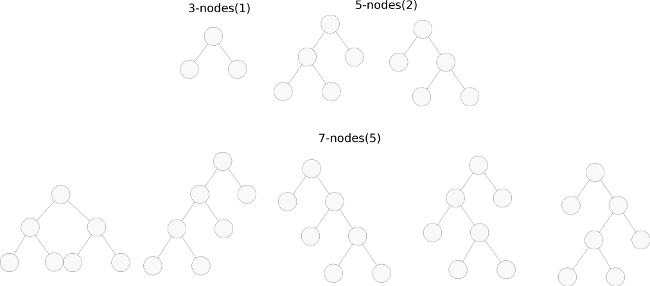
\includegraphics[width=450px, height=225px, keepaspectratio=true]{image/fulltrees.png}
\end{center}

\begin{enumerate}[a)]

\item $B_3 = 1, B_5 = 2, B_7 = 5$.

\item You can't construct a full binary tree with an even number of
  nodes. Every node always has zero or two child nodes, meaning
  everytime the tree grows, it must grow by a multiple of two
  nodes. So starting with the root, and growing $n$ times, the total
  number of nodes will always be of the form $1 + 2n$, which is odd.

\item

  \begin{enumerate}[]
    
  \item Before determining an upper bound for the number of full
    binary trees of some size, it is necessary to know how many leaves
    such a tree has. All full binary trees of size $n$ can be built by
    simply adding two nodes as the left and right child to any leaf
    node on a tree of size $n-2$. For this reason, all full trees with
    the same number of nodes have the same number of leaves.

  \item Considering the full tree with three nodes, it can be seen
    that when nodes are added as the children of a leaf, the new tree
    of size five has one more leaf. This will always be the case,
    because to increase the size of a full tree, it is always
    necessary to add two nodes to a leaf. So the number of leaves on a
    full tree of size $k$ is just the number of times two leaves were
    added to the tree of three nodes plus the original two on that
    tree. So as a function of $k$, the number of leaves of a full tree
    of size $k$, $L_k$, is $L_k = 2 + \frac{k-3}{2}$. The first term is the original
    two leaves on the base tree, and $\frac{k-3}{2}$ is the number of
    times two nodes were added to the base tree.


  \item 
    

  \end{enumerate}

  \[B_n = \left\{
    \begin{tabular}{l r}
      1 & $n \le 3$\\
      2 & $n=5$\\
      5 & $n=7$\\
      $2(B_{n-1} + B_{n-2})$ &  $n > 7$\\
    \end{tabular}
  \right\}\]

\end{enumerate}


\section*{Problem 3}


\begin{verbatim}
  structure weirdqueue {
     pushstack (stack pointer)
     popstack (stack pointer)
  }

  def enqueue(Q, elt):
     Q.pushstack.push(elt)

  def dequeue(Q):
     if Q.pushstack and Q.popstack are empty:
        error underflow
     if Q.popstack is empty:
        while Q.pushstack is not empty:
           Q.popstack.push( Q.pushstack.pop() )
        swap Q.popstack pointer with Q.pushstack
     return Q.popstack.pop()

\end{verbatim}


\begin{enumerate}[a)]

\item Under the assumption that the 'popstack' is empty, we would have
  to pop each element off the 'pushstack' and then push that on to the
  'popstack.' By doing this we are reversing the order, guaranteeing
  that we get the first queued item, but means we are also doing work
  proportional to the size of the structure, $O(n)$.

\item In practice, we could not possibly have to do this mass popping
  and pushing to reorient the structure every dequeue. This means that
  we will have a much faster amortized analysis of the running
  time. If we follow the lifetime of one element in the structure,
  there are only about 4 operations associated with it. We initially
  push it on to the 'pushstack' and then at some later time we will
  transfer it to the 'popstack' and finally pop it one more time when
  it is removed. So there can never be more than 4 operations per
  element lifecycle. Using amortized analysis, we can see that $n$
  insertions could never be worse than about $4n$ stack
  operations. Therefore, the average cost per enqueue/dequeue
  operation is $\frac{4n}{n} = 4$, which is $O(1)$.
  
\end{enumerate}

\end{document}
